% Updated by Michael Gertz, April 2017
%%%%%%%%%%%%%%%%%%%%%%%%%%%%

\documentclass{beamer}
%\usepackage[ngerman]{babel}
\usepackage[utf8]{inputenc}

\usepackage{color}
\usepackage{graphicx}
\usepackage{fancybox}

\usepackage{beamerthemesplit}
\usetheme[compress]{Heidelberg}
\definecolor{unirot}{rgb}{0.5976525,0,0}
\usecolortheme[named=unirot]{structure}


\title[Building Conversational QA-Systems]{Building Conversational \newline Question Answering Systems}
\subtitle{Master's Thesis Presentation}
\author[Stephan Lenert]{Stephan Lenert}
% \date{\today}
\date{April 16, 2024}
\institute[Uni HD]{
Heidelberg University\\
Institute of Computer Science\\
Database Systems Research Group\\
\color{unirot}{stephan.lenert@stud.uni-heidelberg.de}}

%---------------------------------------%
%---------- RECURRING OUTLINE ----------%
% have this if you'd like a recurring outline
\AtBeginSection[]  % "Beamer, do the following at the start of every section"
{
\begin{frame}<beamer> 
\frametitle{Outline} % make a frame titled "Outline"
\tableofcontents[currentsection,hideallsubsections]  % show TOC and highlight current section
\end{frame}
}
%----------------------------------------


\begin{document}
\frame[plain]{\titlepage}
\frame{\frametitle{Outline}\tableofcontents[hideallsubsections]}

%========================================
%========================================

\section[Introduction]{Introduction}

\subsection{Introduction}

\frame{
\frametitle{Introduction}

  \begin{overprint}
  \onslide<1>
  \begin{figure}
  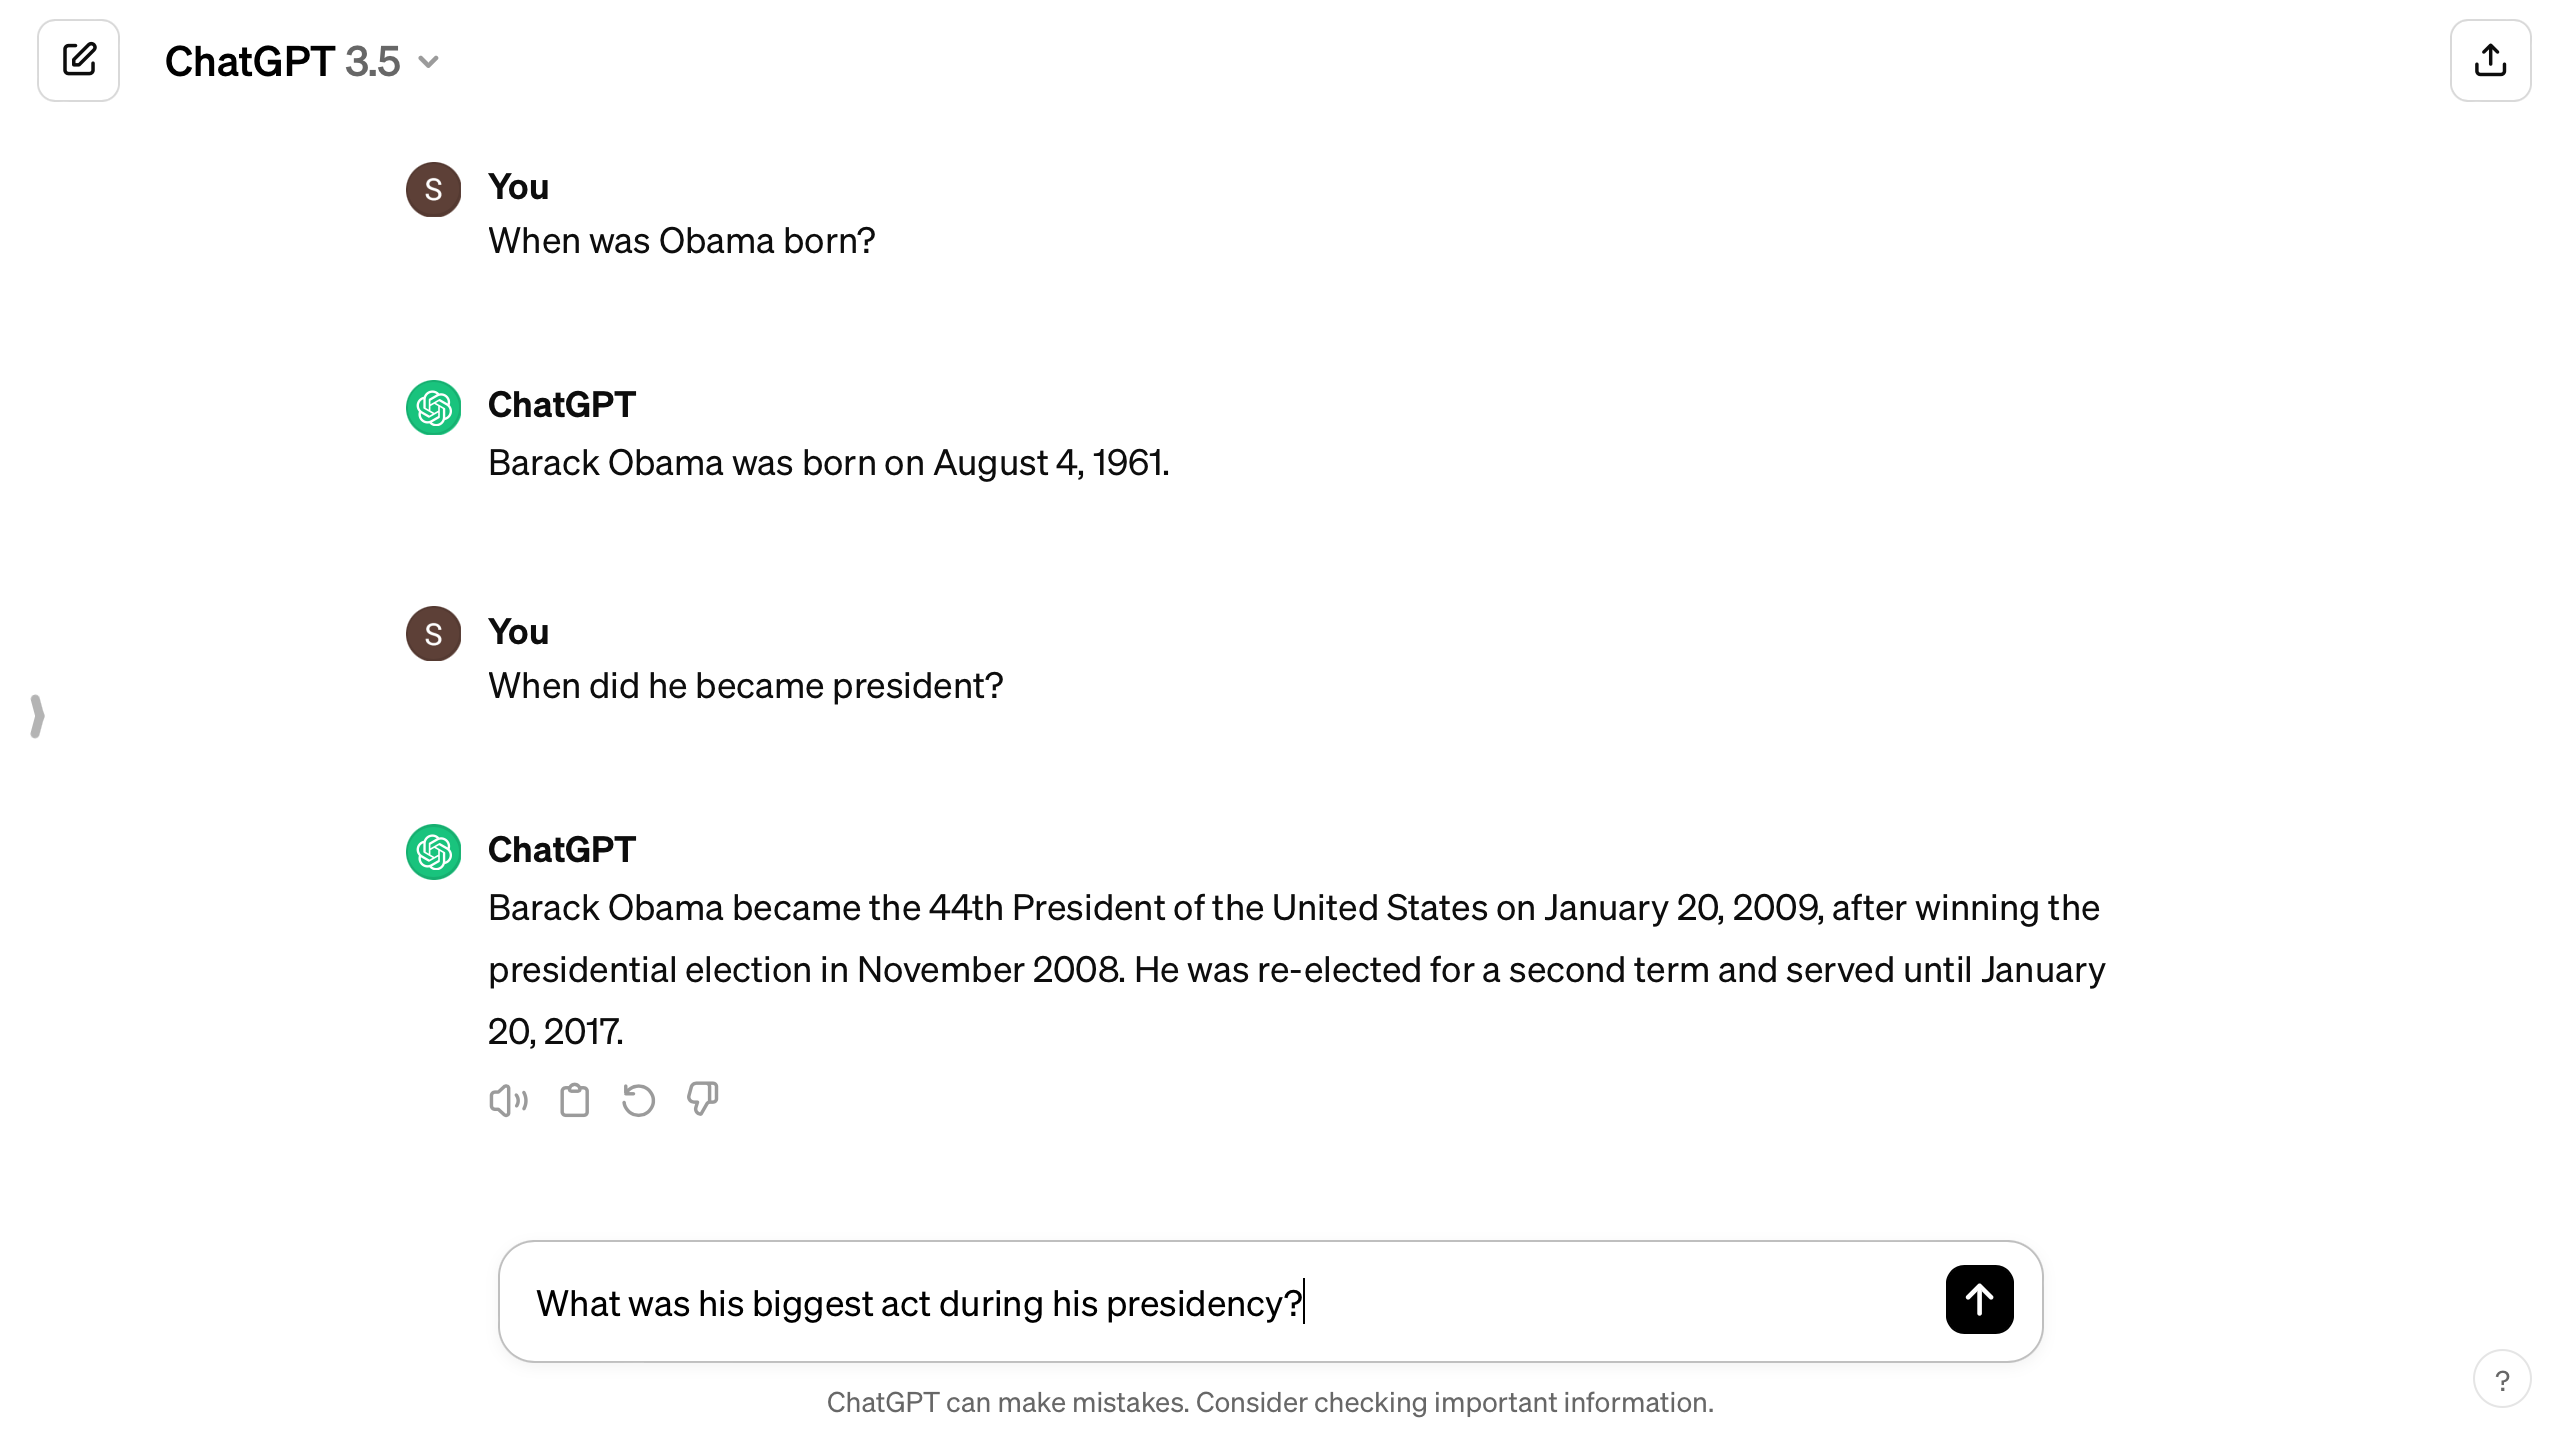
\includegraphics[width=\textwidth]{Grafiken/Obama_Chatgpt.png} 
  \caption{Question Answering with ChatGPT, \textit{Source: chat.openai.com}}
  \end{figure}
  \onslide<2>
  \begin{figure}
  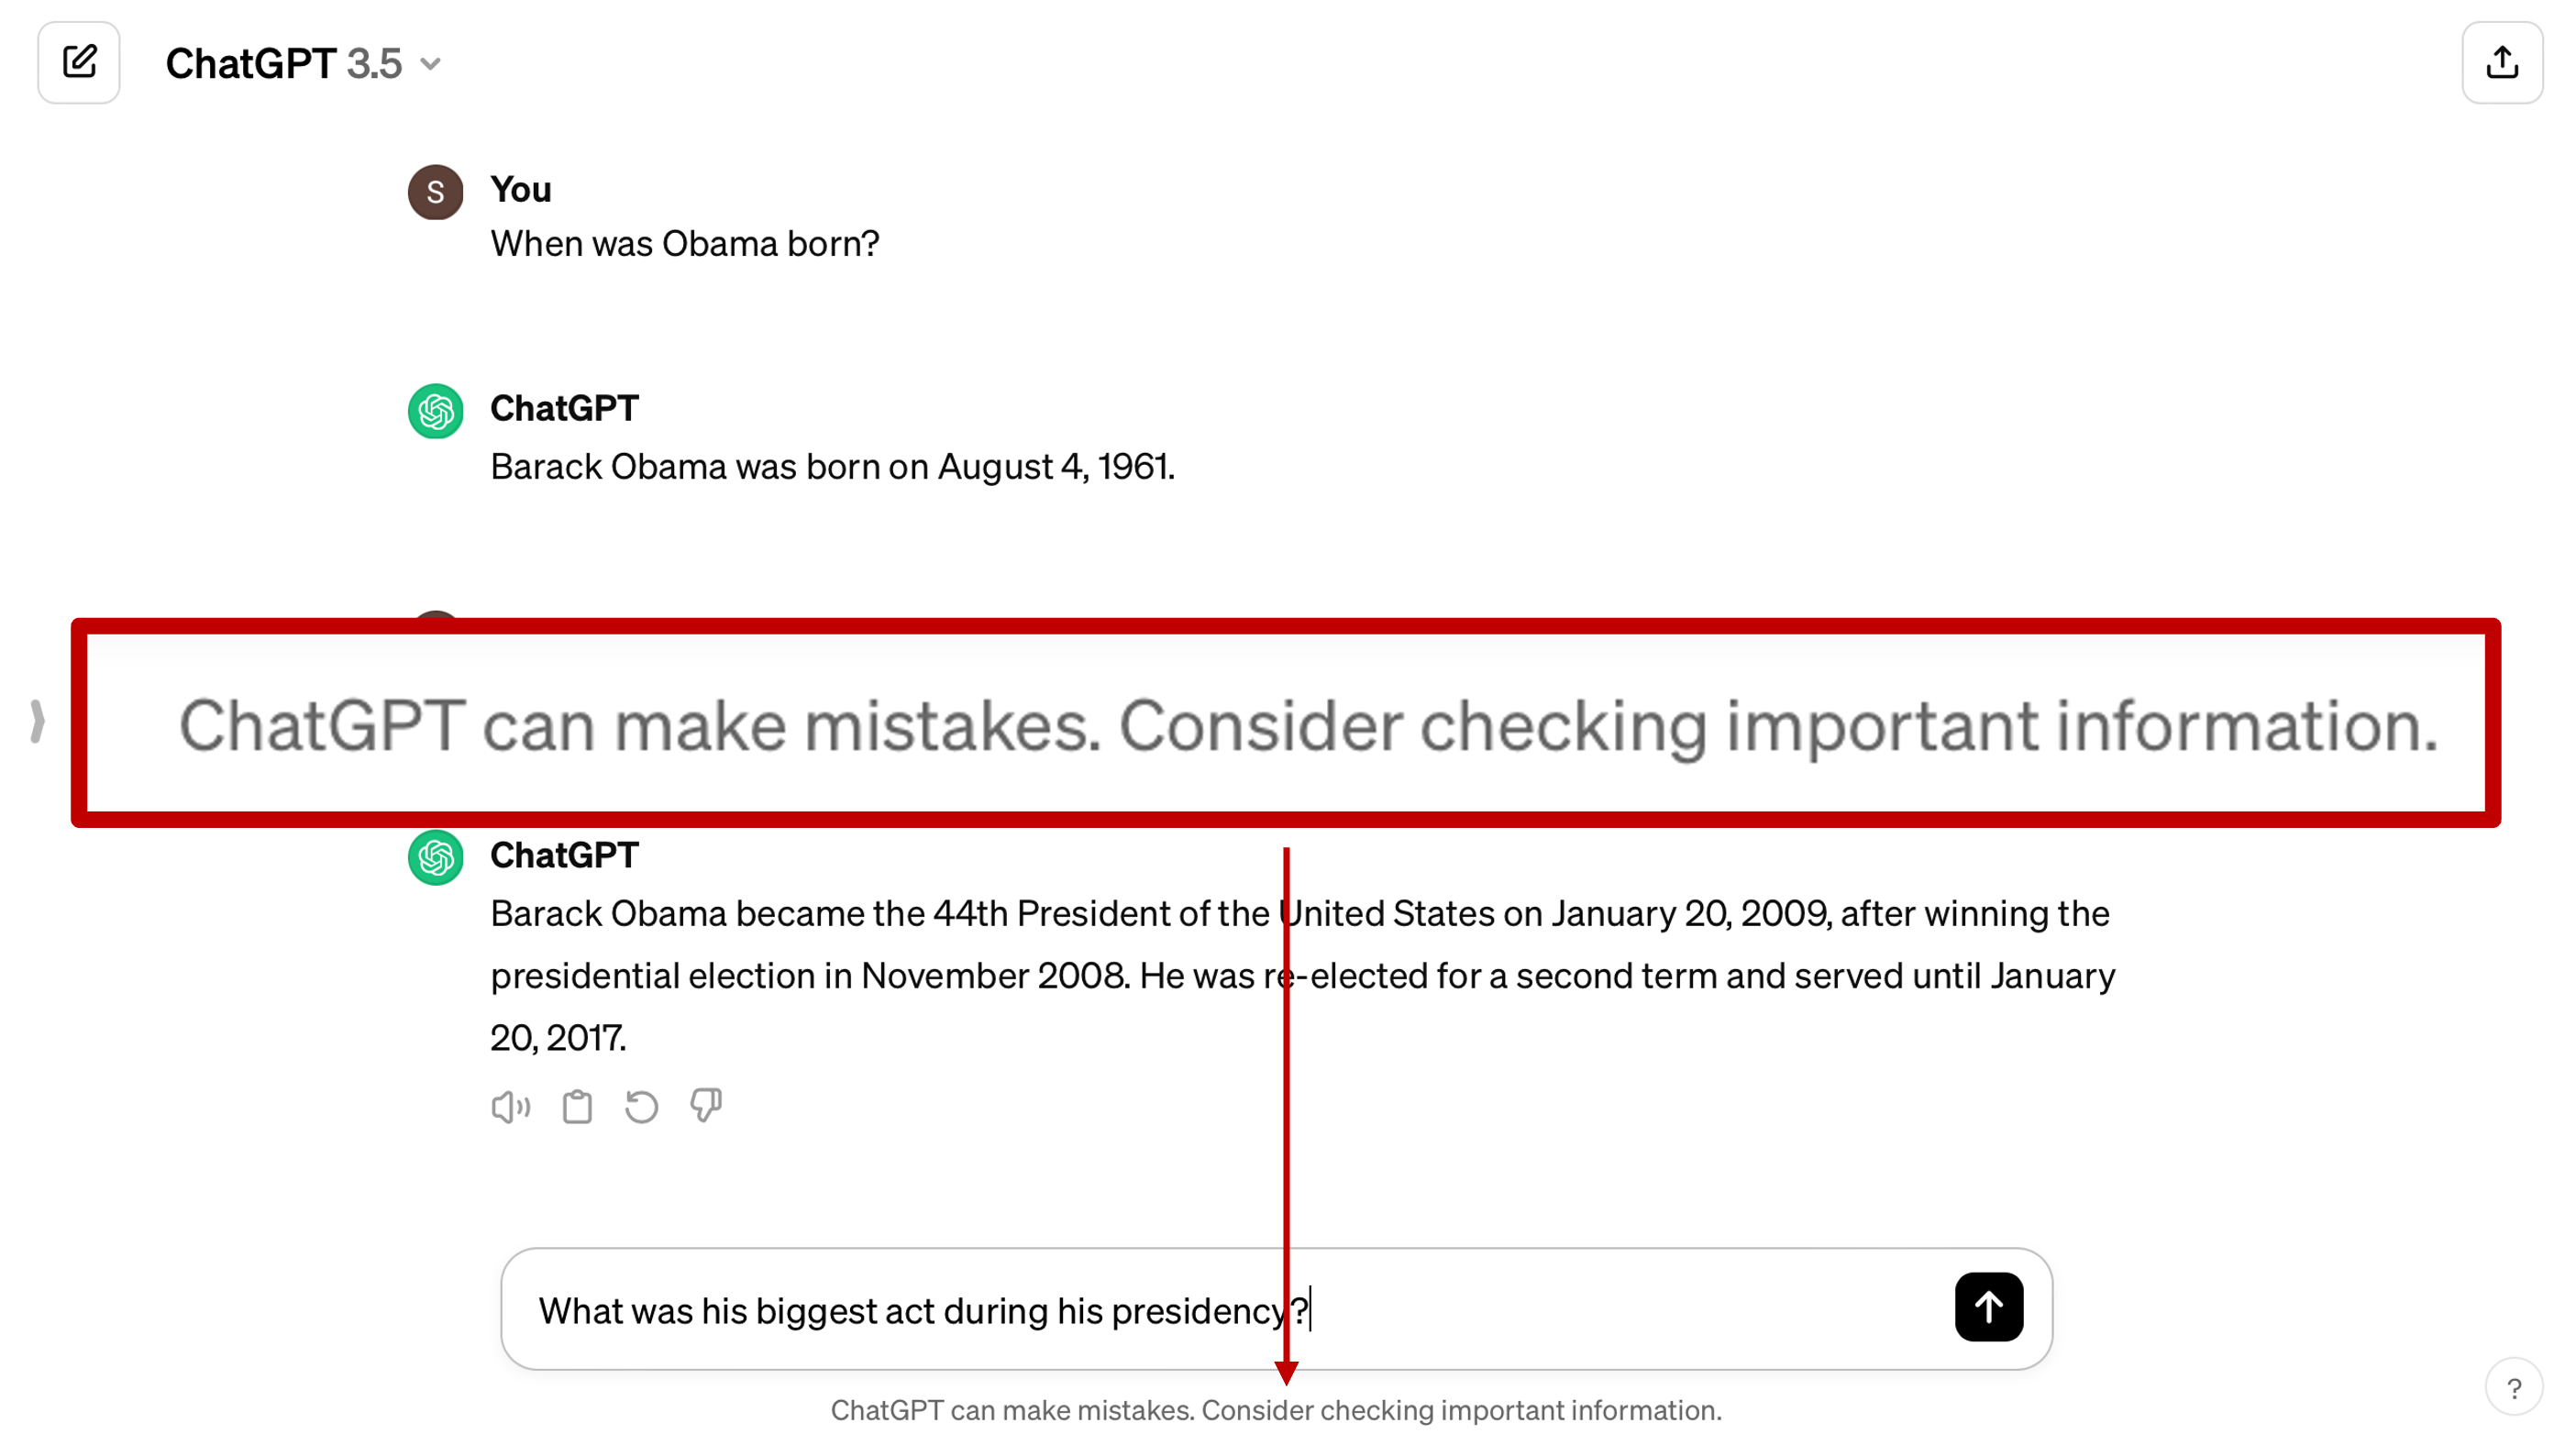
\includegraphics[width=\textwidth]{Grafiken/Chatgpt_Message_Highlight.png}
  \caption{Question Answering with ChatGPT, \textit{Source: chat.openai.com}}
  \end{figure}
  \end{overprint}

}

\frame{
\frametitle{Generative-only QA-Systems}

  {\color{unirot}Issues of generative-only QA-systems:}
  \begin{itemize}
    \item Parameterized Knowledge
    \item Explainability
    \item Hallucination
  \end{itemize}

% Mention Source
  \bigskip
  \textbf{Source:} [Lewis et al., 2020b]  
  \bigskip
}

\frame{
  \frametitle{How to build Use-Case specific QA-Systems?}
  % Three Rows

  \begin{overprint}
  \onslide<1>
    \begin{columns}[t]
    \begin{column}{.5\textwidth}
    {\color{unirot}Research Papers}
    \begin{itemize}
      \item Feng, 2021
      \begin{itemize}
        \item Utilizes visual document question answering
        \item Uses extractive Readers, not the latest LLMs
      \end{itemize}
    \end{itemize}
    \end{column}


    \begin{column}{.5\textwidth}
    {\color{unirot}Frameworks} 
    \begin{itemize}
      \item Langchain
      \begin{itemize}
        \item Bound to explicit RAG approaches
        \item Limited to predefined Extraction, Retriever and Index Tools 
      \end{itemize}
      \item OpenAI Plugins
        \begin{itemize}
          \item Same as Langchain
          \item Limited to ChatGPT
        \end{itemize}
    \end{itemize}
    \end{column}

    \end{columns}
    \vfill
  \onslide<2>
      \begin{columns}[t]
        \begin{column}{.5\textwidth}
        {\color{unirot}Research Papers}
        \begin{itemize}
          \item Feng, 2021
          \begin{itemize}
            \item Utilizes visual document question answering
            \item Uses extractive Readers, not the latest LLMs
          \end{itemize}
        \end{itemize}
        \end{column}
    
    
        \begin{column}{.5\textwidth}
        {\color{unirot}Frameworks} 
        \begin{itemize}
          \item Langchain
          \begin{itemize}
            \item Bound to explicit RAG approaches
            \item Limited to predefined Extraction, Retriever and Index Tools 
          \end{itemize}
          \item OpenAI Plugins
            \begin{itemize}
              \item Same as Langchain
              \item Limited to ChatGPT
            \end{itemize}
        \end{itemize}
        \end{column}
    
        \end{columns}
        \vfill
    \begin{block}{There exists a Research Gap ...}
    No research work explores the use-case specific implementation of conversational question answering systems.
    \end{block}
  \end{overprint}
}

\section[Thesis' Goal]{Goal of the Thesis}

\frame{
\frametitle{Example Use-Case}

\begin{overprint}
\onslide<1>
\begin{figure}
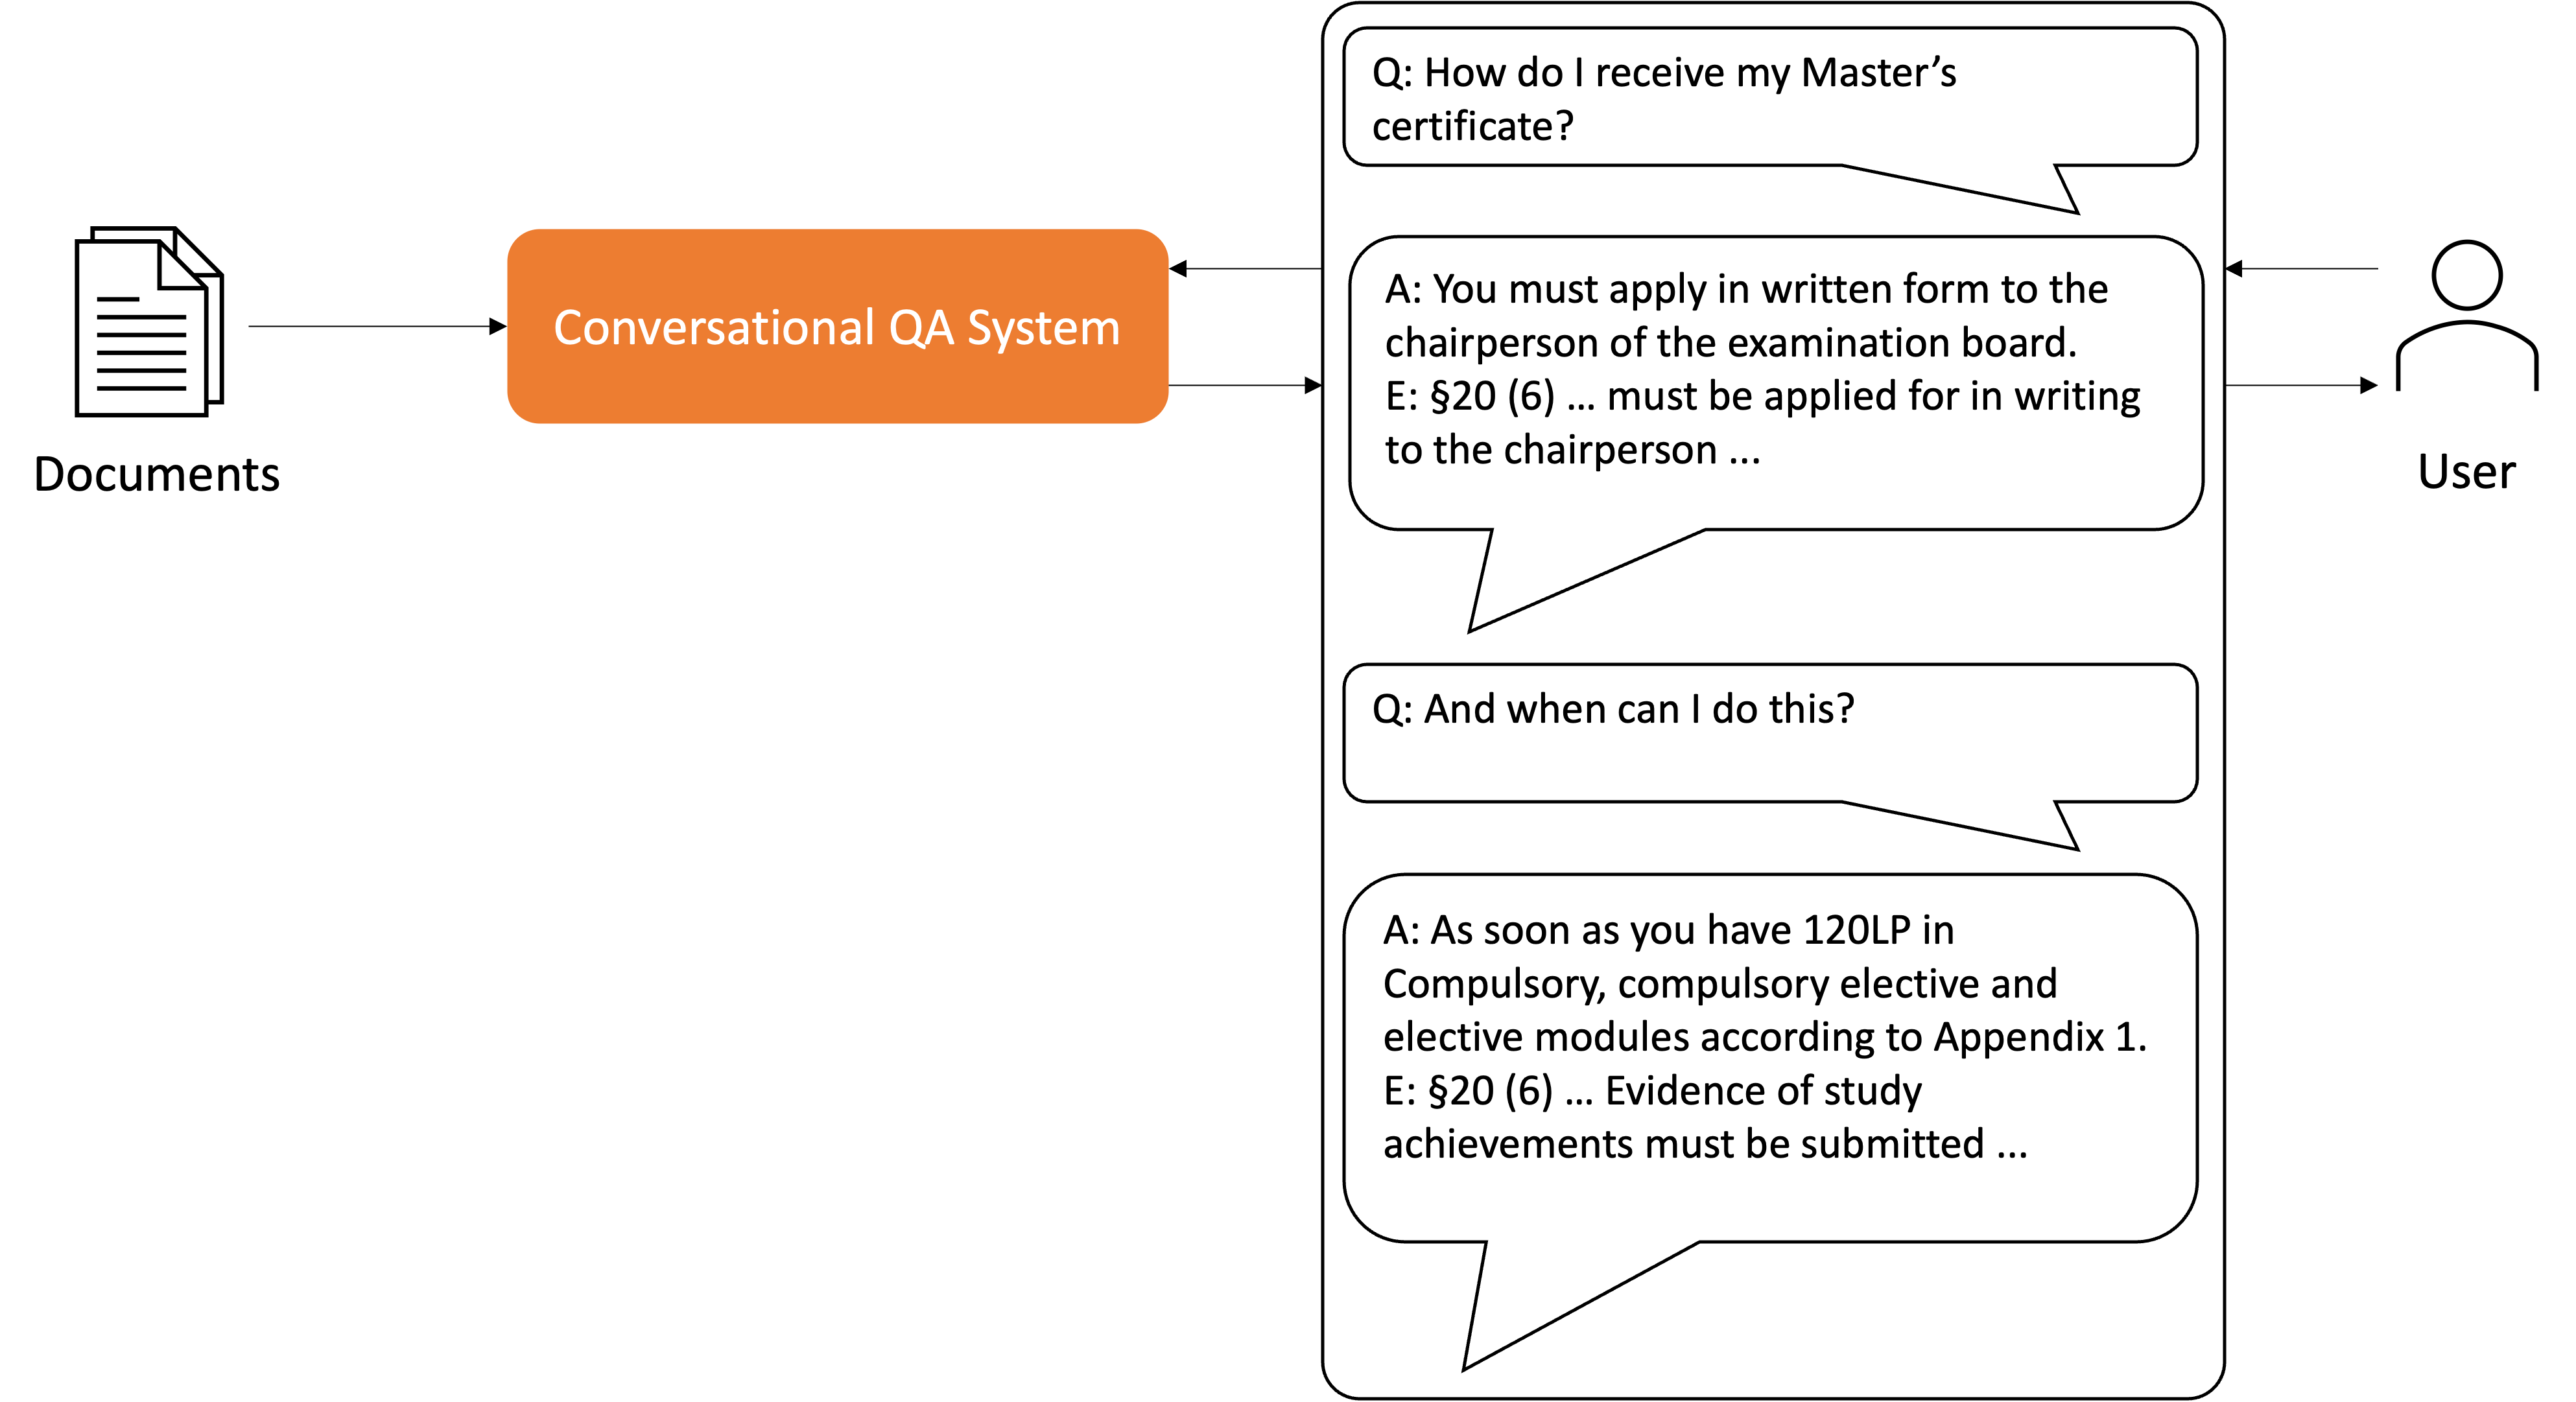
\includegraphics[width=\textwidth]{Grafiken/Use_Case.png}
\caption{Overview of the Example Use-Case}
\end{figure}

\onslide<2>
\begin{figure}
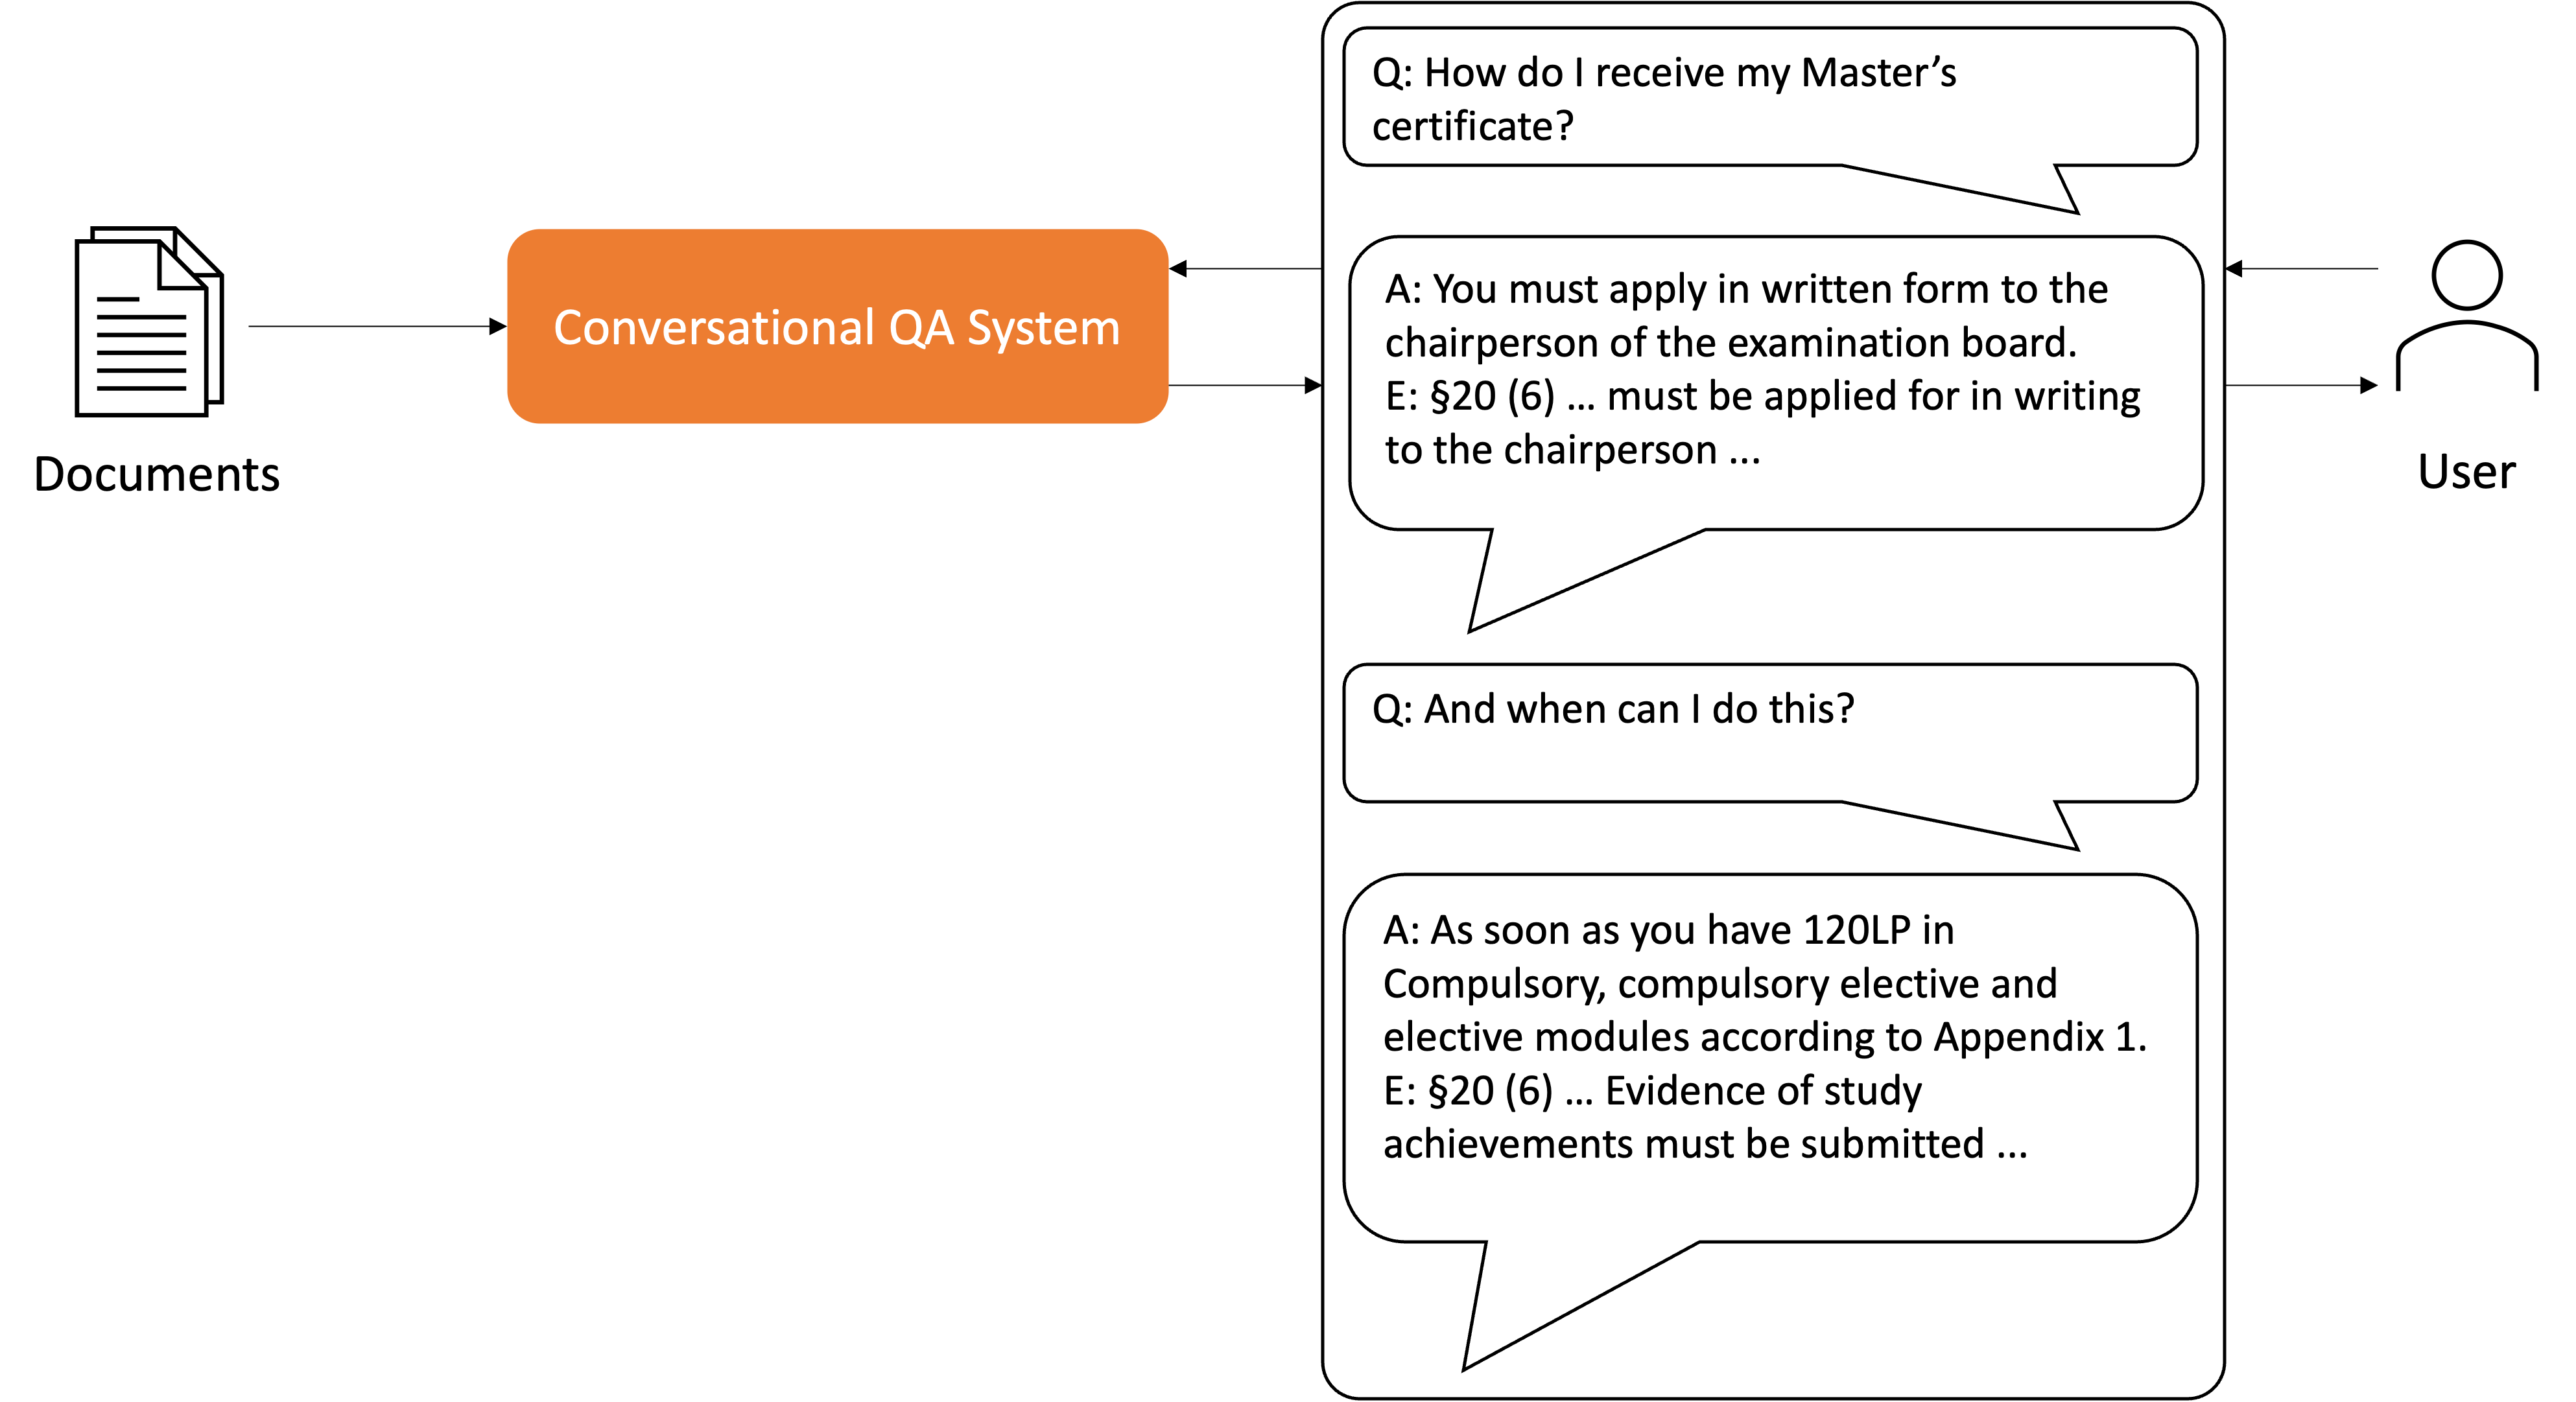
\includegraphics[width=\textwidth]{Grafiken/Use_Case.png}
\caption{Overview of the Example Use-Case}
\end{figure}
\vspace*{-5cm}
\begin{block}{Defined Goal}
  To build a framework for a conversational question-answering system that is tailored to a specific collection of documents.
\end{block}
\end{overprint}
}

\section[Fundamentals]{Fundamental Concepts}

\begin{frame}
  \frametitle{Natural Language QA}

  \begin{figure}
    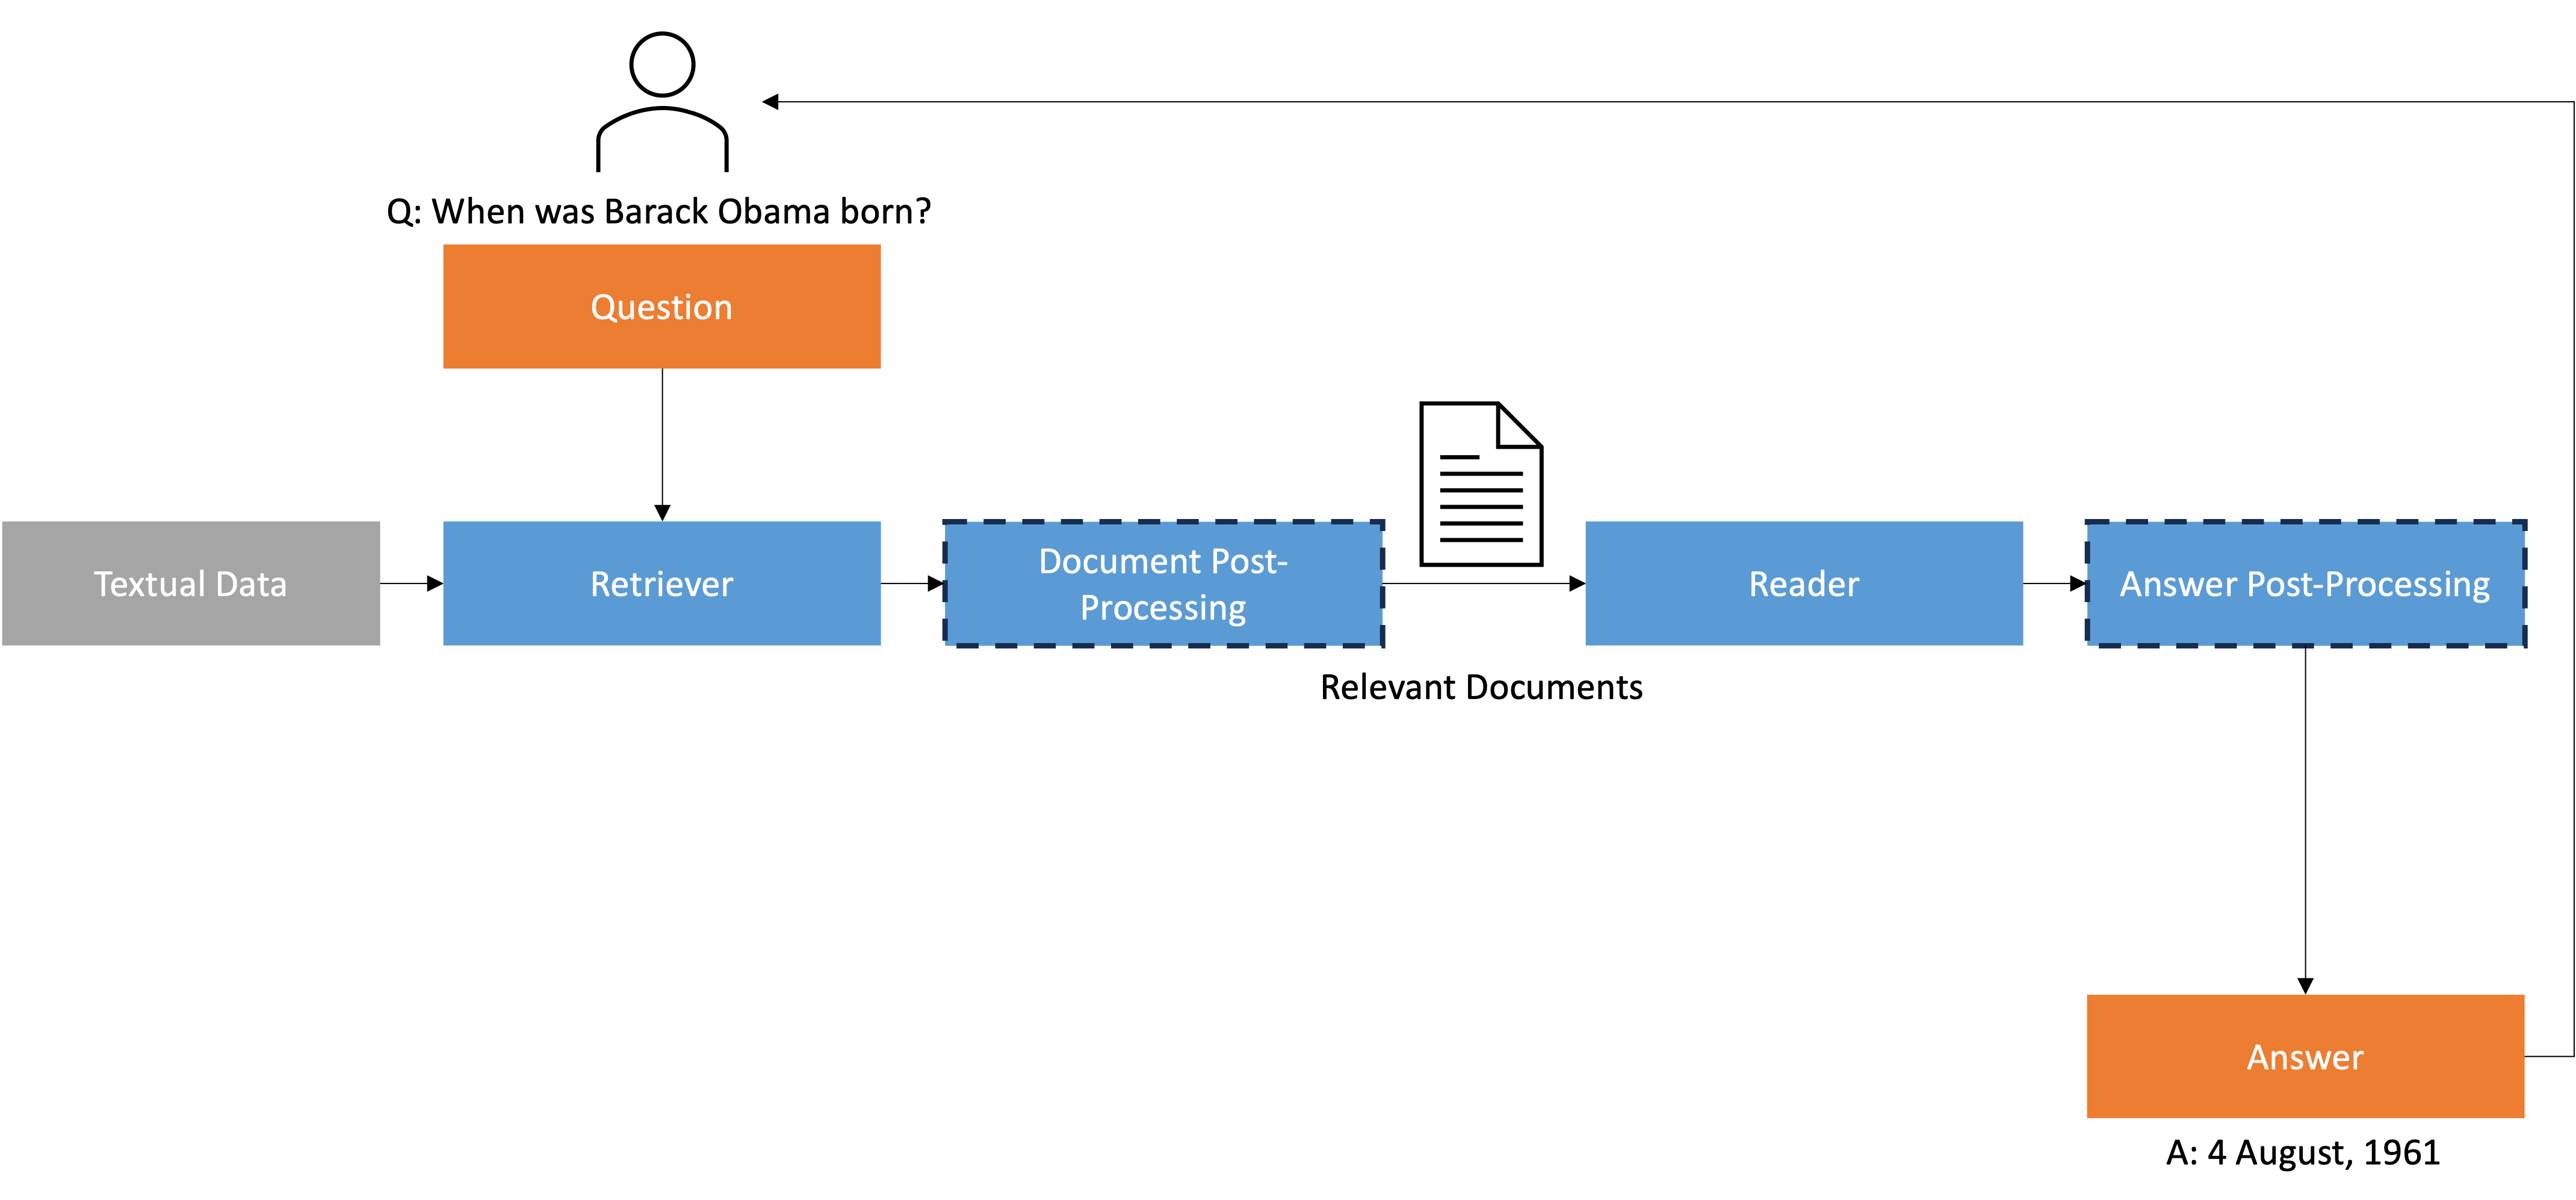
\includegraphics[width=\textwidth]{Grafiken/Retriever_Reader.png}
    \caption{Reader-Retriever-System Architecture for QA by Zhu et al. [Zhu et al., 2021]}
  \end{figure}

\end{frame}

\begin{frame}
  \frametitle{Retriever and Reader}

  % Create two rows retriever and reader
  \begin{columns}[t]
    \begin{column}{.5\textwidth}
    {\color{unirot}Retriever}
    \begin{itemize}
      \item Retrieves relevant documents given a query
      \item Existing approaches
      \begin{itemize}
        \item Sparse Retrieval
        \item Dense Retrieval
        \item Iterative Retrieval
      \end{itemize}
    \end{itemize}
    \end{column}
    \begin{column}{.5\textwidth}
    {\color{unirot}Reader}
    \begin{itemize}
      \item Extracts answers from evidence set given a query
      \item Existing approaches
      \begin{itemize}
        \item Extractive
        \item Generative
      \end{itemize}
    \end{itemize}
    \end{column}
  \end{columns}

\end{frame}

\begin{frame}
  \frametitle{Retrieval-Augmented Generation}

  \begin{figure}
    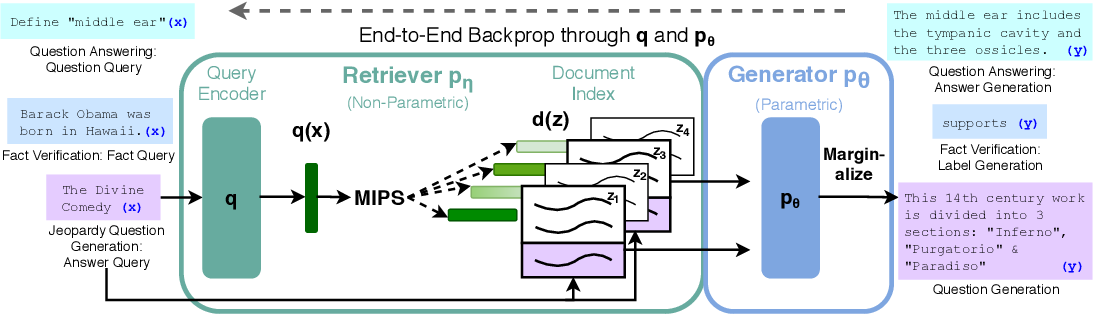
\includegraphics[width=\textwidth]{Grafiken/RAG-Figure1.png}
    \caption{RAG by Lewis et al. [Lewis et al., 2020b]}
  \end{figure}

  RAG:
  \begin{itemize}
    \item Extends parametric knowledge of generator by non-parametric retrieved evidences
    \item Originally proposed as end-to-end training
    \item Modern RAG implementations use explicit evidence sets
  \end{itemize}
  
\end{frame}

\begin{frame}{Conversation}
  
  \begin{columns}[t] % align columns
    \begin{column}{.6\textwidth}
      \vfill
      \begin{figure}
        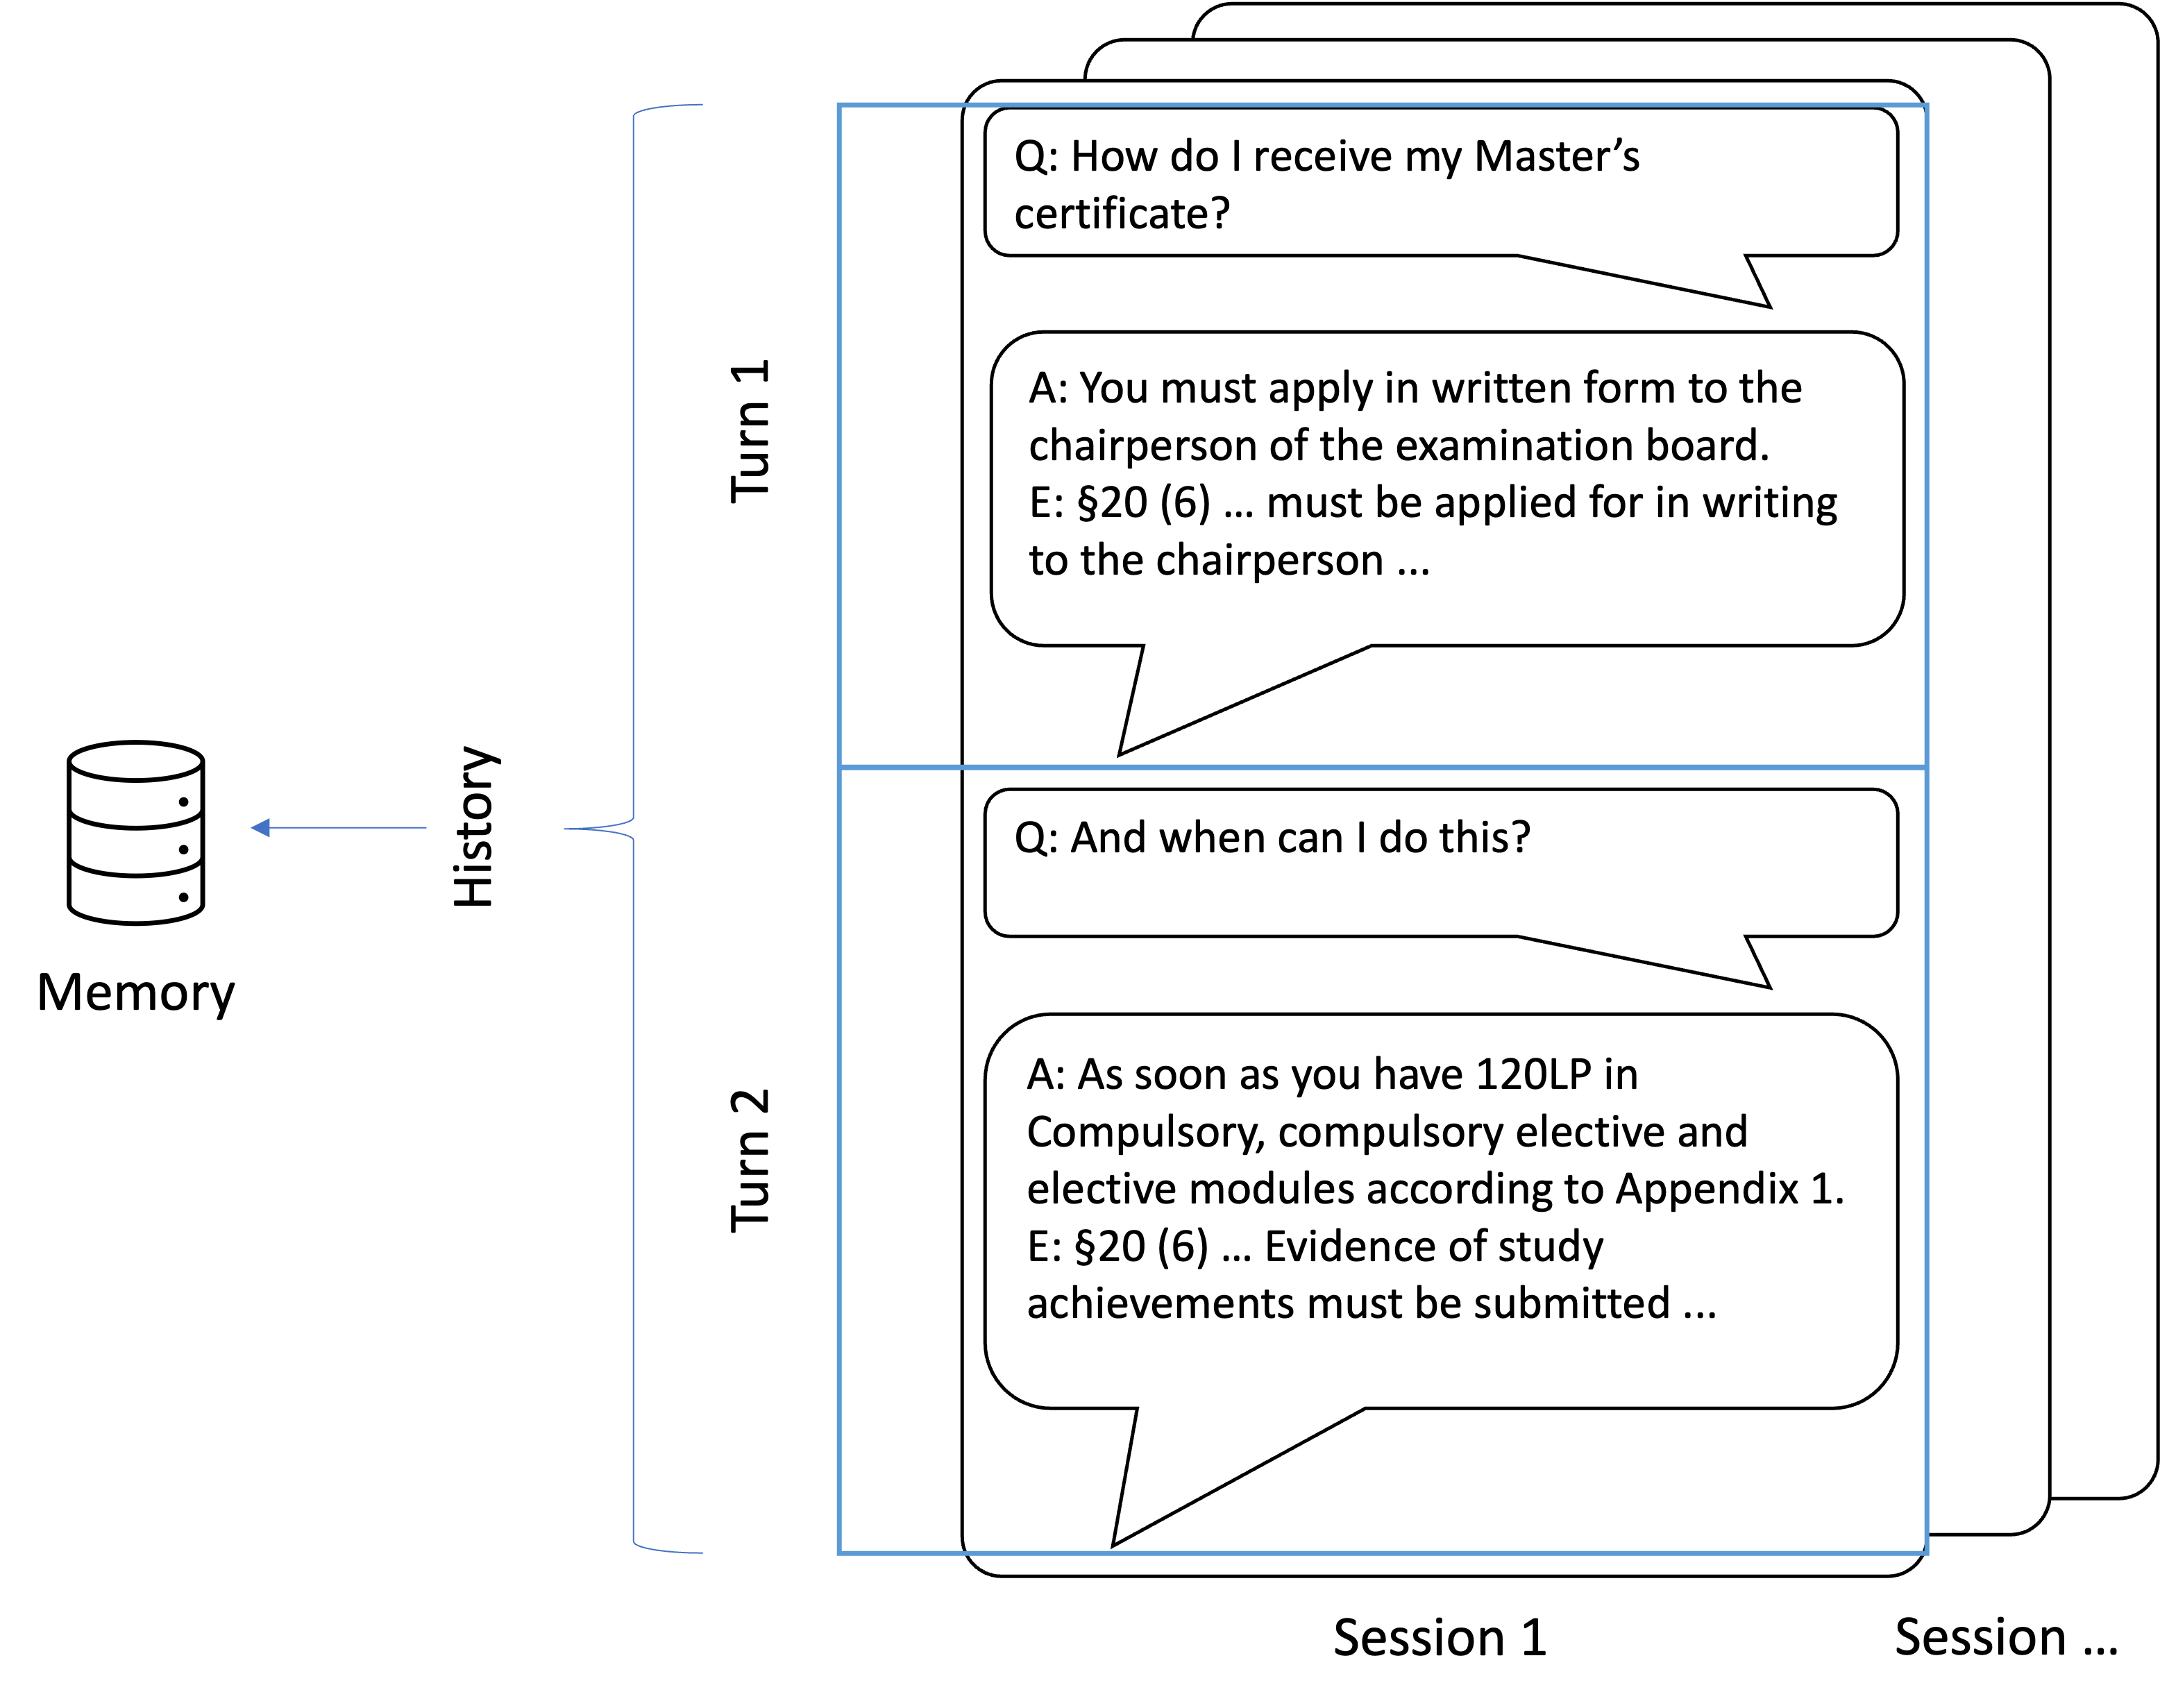
\includegraphics[width=\textwidth]{Grafiken/Conversation_Explain.png}
        \caption{Concepts of a Conversation in regards to a CIS}
      \end{figure}
      \vfill
    \end{column}
    
    \begin{column}{.4\textwidth}
      \vfill
      Important Concepts:
      \begin{itemize}
        \item Turn - A user question and system answer.
        \item History - Previous turns in a session.
        \item Session - A complete conversation.
        \item Memory - System's knowledge of the conversation(s).
      \end{itemize}
      \vfill
    \end{column}
  \end{columns}

\end{frame}

\section[Problem Statement]{Problem Statement}

\begin{frame}{QA-System}
  \begin{enumerate}
    \item Utilize \textbf{documents} as the primary \textbf{knowledge source}.
    \item Enable the QA-System to handle a \textbf{variety of answer types}, including: \textbf{extractive}, \textbf{abstractive}, and \textbf{boolean}.
    \item \textbf{Provide references} to document snippets \textbf{as evidence to answers}.
    \item Ensure the pipeline's generalizability by using \textbf{open-domain methods}, allowing it to adapt to new domains or knowledge sources with \textbf{minimal or no supervision} and \textbf{small datasets}.
    \item Design the pipeline to be \textbf{feasible without the need for datacenter-grade hardware resources}, making it accessible for development on standard research hardware.
  \end{enumerate}
\end{frame}
  
\begin{frame}{QA-System (cont.) and Conversationality}
  \begin{enumerate}
    \setcounter{enumi}{5}
    \item \textbf{Prioritize accuracy as the primary objective}, as constraining memory consumption is indirectly covered in point (5). \textbf{Latency is not a primary concern}, as the system is not intended for real-time use and will not be optimized for that in this thesis.
  \end{enumerate}
  
  Conversationality:
  \begin{enumerate}
    \item Enable the ConvQA-System to \textbf{handle} the following follow-up \textbf{question types: drilling-down, clarification, topic shift} and \textbf{comparison}.
    \item Be able to take Initiative in the form of \textbf{clarifying questions}.
    \item The \textbf{memory} will be \textbf{limited to a session} and not multi-session.
  \end{enumerate}
\end{frame}

\section[ConRAG]{ConRAG}

\section[Implementation]{Implementation}

\section[Experiments]{Experiments}

\section[Results]{Results}

% \section[Structure]{Page Structure}

% \subsection{Enumerations}


% \frame{
% \frametitle{Enumerations}

% \begin{itemize}
% \item Item
% \begin{itemize}
%   \item Subitem 1
%   \item Subitem 2
%   \item Subitem 3
% \end{itemize}
% \item Another main item
% \item And yet another one
% \begin{itemize}
%   \item \ldots with subitem
% \end{itemize}
% \end{itemize}
% } % END OF FRAME

% %----------------------------------------

% \frame{
% \frametitle{Enumerations / 2}

% \begin{itemize}
% \item Item
% \medskip
% \begin{itemize}
%   \item Subitem 1
%   \medskip
%   \item Subitem 2
%   \medskip
%   \item Subitem 3
% \end{itemize}
% \bigskip
% \item And another item
% \bigskip
% \item And yet another one
% \medskip
% \begin{itemize}
%   \item again with subitem
% \end{itemize}
% \end{itemize}
% } % END OF FRAME

% %----------------------------------------

% \frame[t]{
% \frametitle{Enumerations / 3}

% \begin{itemize}
% \item Main item with 3 subitems
% \begin{itemize}
%   \item[(a)] Subitem 1
%   \item[(b)] Subitem 2
%   \item[(c)] Subitem 3
% \end{itemize}
% \item And another item
% \item And yet another one
% \begin{itemize}
%   \item \ldots again with subitem 
% \end{itemize}
% \end{itemize}
% } % END OF FRAME

% %========================================

% \subsection{Rows}


% \frame{
% \frametitle{Rows}

% \begin{columns}[t]
% \begin{column}{.5\textwidth}
% {\color{unirot}Advantages}
% \begin{itemize}
%   \item There are many
%   \item and more
%   \item and even more
%   \item and a last advantage
% \end{itemize}
% \end{column}


% \begin{column}{.5\textwidth}
% {\color{unirot}Disadvantages} 
% \begin{itemize}
%   \item There is only one 
%   \item or two
% \end{itemize}
% \end{column}

% \end{columns}
% \vfill
% } % END OF FRAME

% %----------------------------------------

% \frame{
% \frametitle{Rows / 2}

% \begin{columns}[b]
% \begin{column}{.5\textwidth}
% {\color{unirot}Advantages}
% \begin{itemize}
%    \item There are many
%   \item and more
%   \item and even more
%   \item and a last advantage
% \end{itemize}
% \end{column}


% \begin{column}{.5\textwidth}
% {\color{unirot}Disadvantages} 
% \begin{itemize}
%   \item There is only one 
%   \item or two
% \end{itemize}
% \end{column}

% \end{columns}
% \vfill
% } % END OF FRAME

% %========================================

% \subsection{Blocks}


% \frame{
% \frametitle{Blocks}

% \begin{block}{\centering Definition of x}
% x is an important parameter for any type of text.
% \end{block}

% \medskip
% \begin{block}{\centering Steps}
% \begin{itemize}
%   \item[(1)] Practice
%   \item[(2)] Practice
%   \item[(3)] Practice
% \end{itemize}
% \end{block}

% \medskip
% \begin{block}{}
% \centering

% A block does not require a title.
% \end{block}

% } % END OF FRAME



% %========================================
% %========================================

% \section[Transitions]{Transitions  between Slides}

% \subsection{Simpel pause and the like}


% \frame{
% \frametitle{Enumerations}

% \begin{itemize}
% \item Main item
% \begin{itemize}
%   \item Subitem 1
%   \item Subitem 2
%   \item Subitem 3
% \end{itemize}
% \pause

% \item Another main item
% \pause

% \item And yet another one
% \begin{itemize}
%   \item again with subitem
%   \pause
%   \item and a second subitem
% \end{itemize}
% \end{itemize}
% } % END OF FRAME

% %----------------------------------------

% \frame{
% \frametitle{Enumerations / 2}

% \begin{itemize}
% \item Main item
% \begin{itemize}
%   \item<1> Subitem 1
%   \item<2-3> Subitem 2
%   \item<3-> Subitem 3
% \end{itemize}
% \item<4> Another main item
% \item<4-> And yet another one
% \begin{itemize}
%   \item<6-> again with subitem
%   \item<7> and a second subitem
% \end{itemize}
% \end{itemize}
% } % END OF FRAME

% %========================================

% \subsection{Overlays}

% \frame{
% \frametitle{Overlay of Images}
% \vspace*{-2ex}

% \begin{overprint}
% \onslide<1>
% \begin{figure}
% 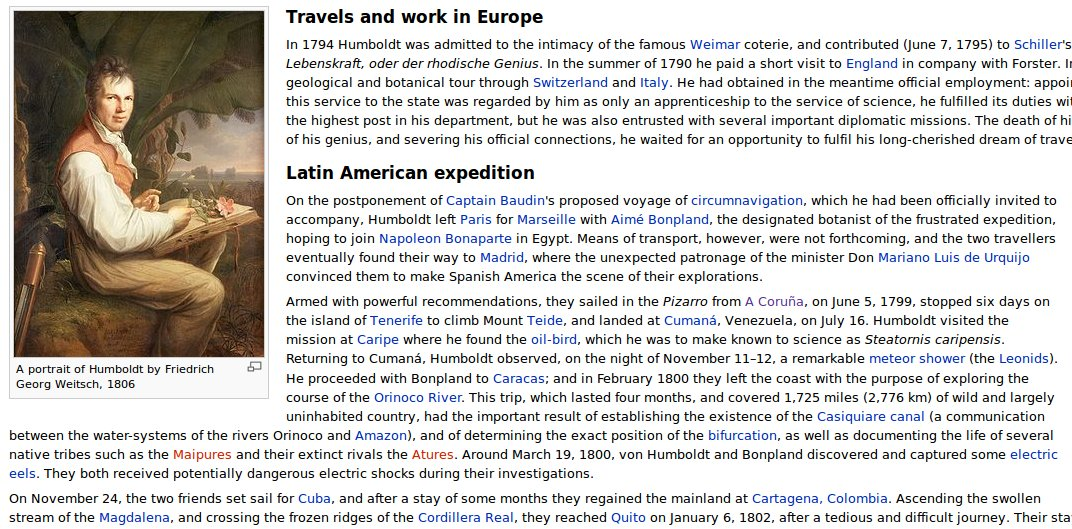
\includegraphics[width=\textwidth]{humboldt_wiki-blank.png} 
% \caption{AvH in Wikipedia, \textit{Source: URL}}
% \end{figure}

% \onslide<2>
% \begin{figure}
% 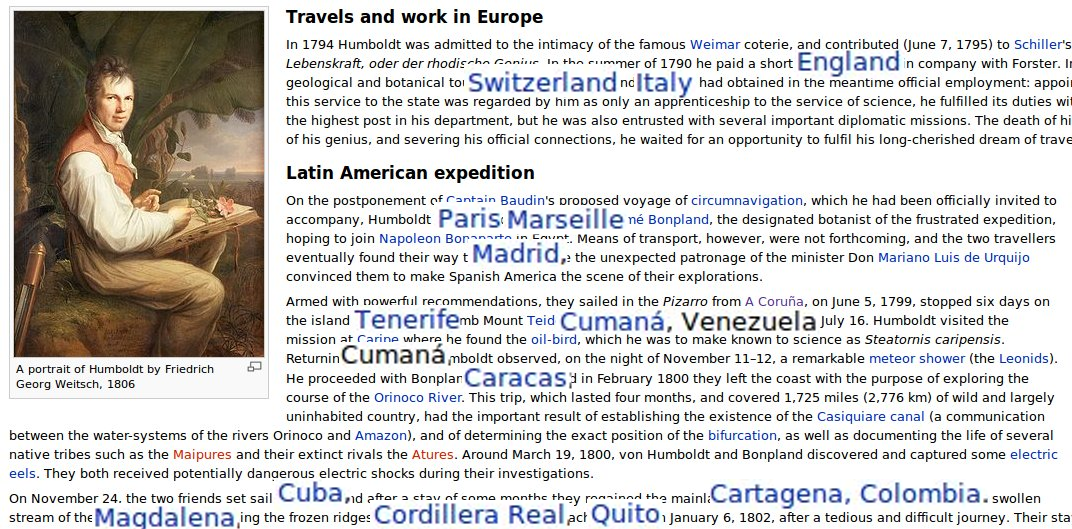
\includegraphics[width=\textwidth]{humboldt_wiki-locations.png} 
% \caption{AvH in Wikipedia, \textit{Source: URL}}
% \end{figure}

% \onslide<3>
% \begin{figure}
% 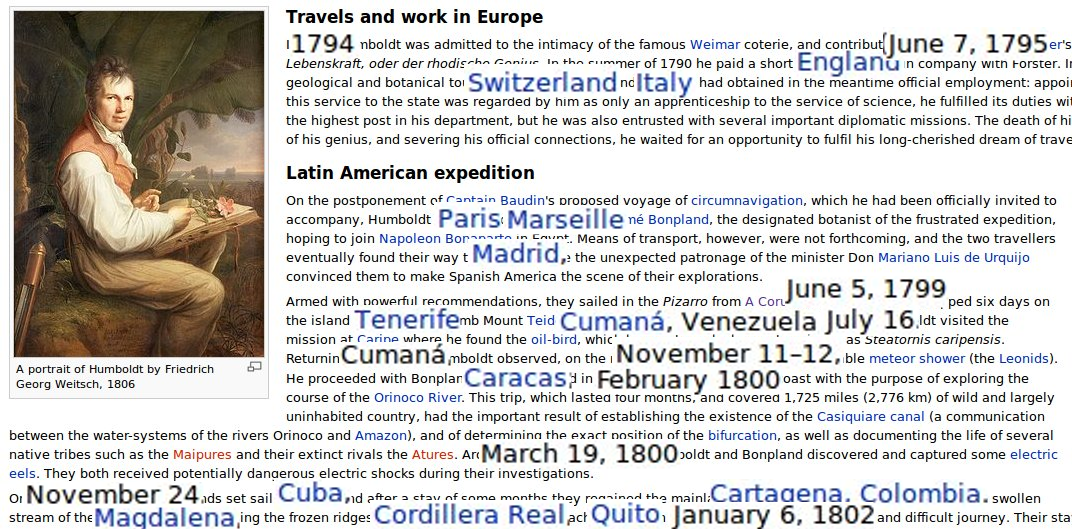
\includegraphics[width=\textwidth]{humboldt_wiki-locations-dates.png} 
% \caption{AvH in Wikipedia, \textit{Source: URL}}
% \end{figure}

% \onslide<4>
% \begin{figure}
% 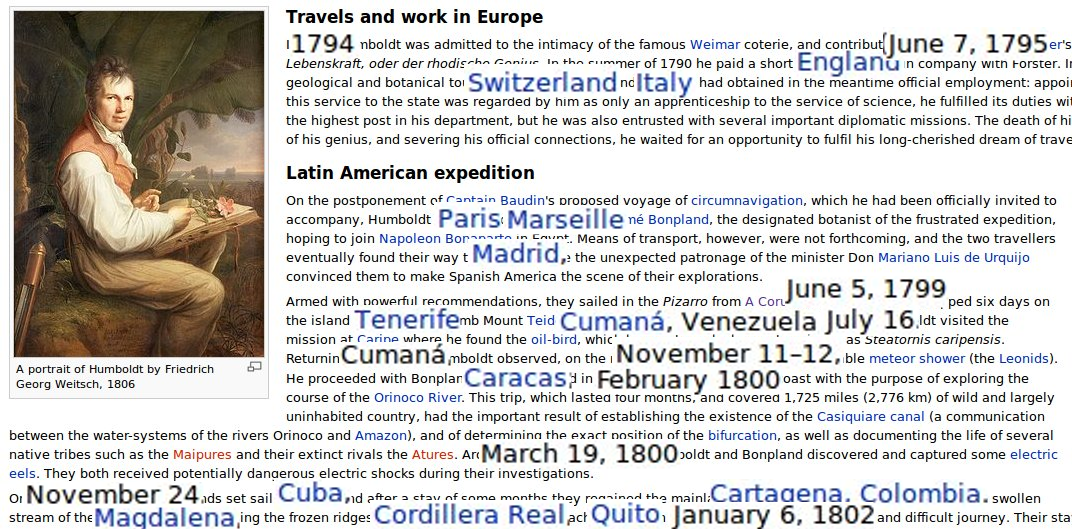
\includegraphics[width=\textwidth]{humboldt_wiki-locations-dates.png} 
% \caption{AvH in Wikipedia, \textit{Source: URL}}
% \end{figure}
% \vspace*{-5cm}
% \begin{block}{An the essence is \ldots}
% \textbf{There were many events in the life of AvH.}
% \end{block}

% \end{overprint}

% } % END OF FRAME

% %----------------------------------------



% \frame{\frametitle{Overlaying Details}
% \vspace*{-1ex}
% \begin{itemize}
% \item What are the issues?
% \begin{overprint}
% \onslide<1>
%   \begin{itemize}
%   \item Issue 1
%   \item Issue 2
%   \item Issue 3
%   \end{itemize}
% \onslide<2>
%   \begin{itemize}
%   \item Issue 1 \\
% \vspace*{-3ex}  
%   \begin{center}
% \includegraphics[width=.3\textwidth]{questions}
% \end{center}
%   \item Issue 2
%   \item Issue 3
%   \end{itemize}
% \onslide<3>
%   \begin{itemize}
%   \item Issue 1
%   \item Issue 2 \\
%   \begin{center}
%   \includegraphics[width=.3\textwidth]{questions}
%   \end{center}
%   \item Issue 3
%   \end{itemize}
% \onslide<4>
%   \begin{itemize}
%   \item Issue 1
%   \item Issue 2
%   \item Issue 3 \\
%   \begin{center}
%   \includegraphics[width=.3\textwidth]{questions}
%   \end{center}
%   \end{itemize}
% \end{overprint}
% \end{itemize}
% } % END OF FRAME



% %========================================
% %========================================

% \section{Accentuations}

% \subsection{Accentuations}

% %----------------------------------------

% \def\hilite<#1>{%
%   \temporal<#1>{\color{black}}{\color{unirot}}%
%                {\color{gray}}}
               
% %----------------------------------------

% \frame{
% \frametitle{Accentuating Parts of Text }

% \textbf{Source:} Beamer v3.0 Guide
% \bigskip

% \begin{Large}
% \begin{tabular}{|p{3.5cm}|}
% \hline
% \texttt{{\hilite<4>A}( Id,{ \hilite<2>X}, {\hilite<3>Y})} \\
% \texttt{B( Id, {\hilite<2>X}, {\hilite<3>Y})} \\ 
% \hline
% \end{tabular}
% \end{Large} 

% } % END OF FRAME

% %----------------------------------------

% \frame{
% \frametitle{Accentuating Parts of Text / 2}

% \textbf{Source:} Beamer v3.0 Guide

% \bigskip
% \begin{itemize}
% \item<1-2> \alert<1>{This is important}
% \item \alert<2-3>{Now this is important}
% \item \alert<3>{Now both are important}
% \item This is never important
% \end{itemize}

% } % END OF FRAME


% %========================================
% %========================================

% \section[More]{More Information}

% \subsection{More Information}

% \frame{
% \frametitle{Useful Beamer Tutorials}

% \begin{itemize}
% \item The Beamer class -- CTAN\\
% \url{http://ctan.math.utah.edu/ctan/tex-archive/macros/latex/contrib/beamer/doc/beameruserguide.pdf}
% \item ``A Beamer Tutorial in Beamer'' von Charles T. Batts \\
% \url{https://www.uncg.edu/cmp/reu/presentations/Charles\%20Batts\%20-\%20Beamer\%20Tutorial.pdf}
% %\texttt{http://www.uncg.edu/cmp/reu/presentations/Charles \\ \%20Batts\%20-\%20Beamer\%20Tutorial.pdf}
% \medskip
% \item The Beamer class for \LaTeX\\
% \url{http://www.mathematik.uni-leipzig.de/~hellmund/LaTeX/beamer2.pdf}
% \medskip
% \item Beamer Theme Matrix \\
% \texttt{http://www.hartwork.org/beamer-theme-matrix/}
% \end{itemize}

% }

% %----------------------------------------

% \frame{\frametitle{Questions}
% \begin{figure}
% \includegraphics[width=.8\textwidth]{questions} 
% \end{figure}
% \vspace*{-3.3cm}\begin{center}\begin{LARGE}\textbf{Questions}\end{LARGE}\end{center}

% \vspace*{2cm}
% }

\end{document}
